\section{Evaluation}  %4 pages
\label{sec:evaluation}


\subsection{Experiment Setup} 
\label{sec:setup}

\subsubsection{Hardware and Software Platforms} 

We evaluate STOF on two generations of GPUs, including NVIDIA RTX 4090 of Ada model and NVIDIA A100 of Ampere model. The experiments are conducted in the software environment configured with Ubuntu 22.04, CUDA v12.6, and PyTorch 2.7.0. We package Docker containers to quickly migrate the software environment between hardware platforms.
% Ubuntu 22.04 或许可以不说 刚好写满 7 行
% The GPU hardware specifications are presented in Table~\ref{tab:hardware}. 

% \begin{table}[htbp]
% \renewcommand{\arraystretch}{1.2}
% \centering
% \caption{Hardware specifications.}
% %\vspace{-5pt}
% % \footnotesize
% \scriptsize
% % \tiny
% \begin{tabular}{l||l|l}
% \hline
%             & \multicolumn{1}{c|}{\textbf{GPU1}}   & \multicolumn{1}{c}{\textbf{GPU2}}                 \\ \hline \hline
% Model       & NVIDIA RTX 4090 (Ada) &  NVIDIA A100 SXM (Ampere) \\ \hline
% % Frequency   & 1.4GHz             & 1.5GHz              \\ \hline
% Cores       & 16,384 (128 SMs)   &   6,912 (108 SMs) \\ \hline
% %Max Warps   & 64 (per SM)       & 48 (per SM)        \\ \hline
% \tabincell{l}{L1 Cache/\\Shared Memory}   & 128KB (per SM)     & 192KB (per SM)     \\ \hline
% L2 Cache    &  72MB             &  40MB             \\ \hline
% Memory      &   24GB GDDR6X      &   40GB HBM2e      \\ \hline
% Bandwidth   & 1,008GB/s       &    1,555GB/s        \\ \hline
% \end{tabular}
% \label{tab:hardware}
% \end{table}


\subsubsection{Comparison Configurations and Methods}


We conduct evaluation on both atomic and compound masking patterns including causal, sliding window, Longformer~\cite{beltagy2020longformer}, and Bigbird~\cite{zaheer2020big}. The sequence length ranges from 128 to 4,096 with a stride of 2$\times$, and the batch size ranges from 1 to 16. For MHA computation, we follow the configuration of BERT-Base. For end-to-end inference, the configuration is set to be consistent with the standard models of BERT~\cite{devlin2019bert}, GPT2~\cite{radford2019language}, LLaMA~\cite{touvron2023llama}, T5~\cite{Raffel2020T5} and ViT~\cite{dosovitskiy2021vit}. We compare STOF with PyTorch Native, PyTorch Compile~\cite{ansel2024pytorch}, FlashAttention2 (FA2)~\cite{dao2023flashattention2}, FlexAttention~\cite{dong2024flex}, ByteTransformer~\cite{zhai2023bytetransformer}, Bolt~\cite{xing2022bolt},  MCFuser~\cite{zhang2024mcfuser}, and SPLAT~\cite{gupta2025splat}. Note that FlexAttention, FA2, and SPLAT are optimized only for MHA, while PyTorch Compile integrates FA2 for MHA computation. In addition, Bolt has no MHA-specific optimizations and only appears in the end-to-end evaluation. Since SPLAT is not open source, we reproduce it based on the contents in the paper. We adopt the half precision (FP16) for evaluation, which is commonly used for model inference in industry~\cite{aminabadi2022deepspeed}, ensuring a unified comparison across all methods. To minimize machine errors, we perform warm-ups for all experiments and run 100 times to record the average performance.

%Considering that the original method of SPLAT is mainly aimed at single precision (FP32), we reproduce SPLAT based on the content described in its paper and adapt it to the half precision (FP16), which is commonly used for model inference in industry~\cite{aminabadi2022deepspeed}, to ensure a unified comparison across all methods.



\begin{figure*}[htbp]
    \centering
    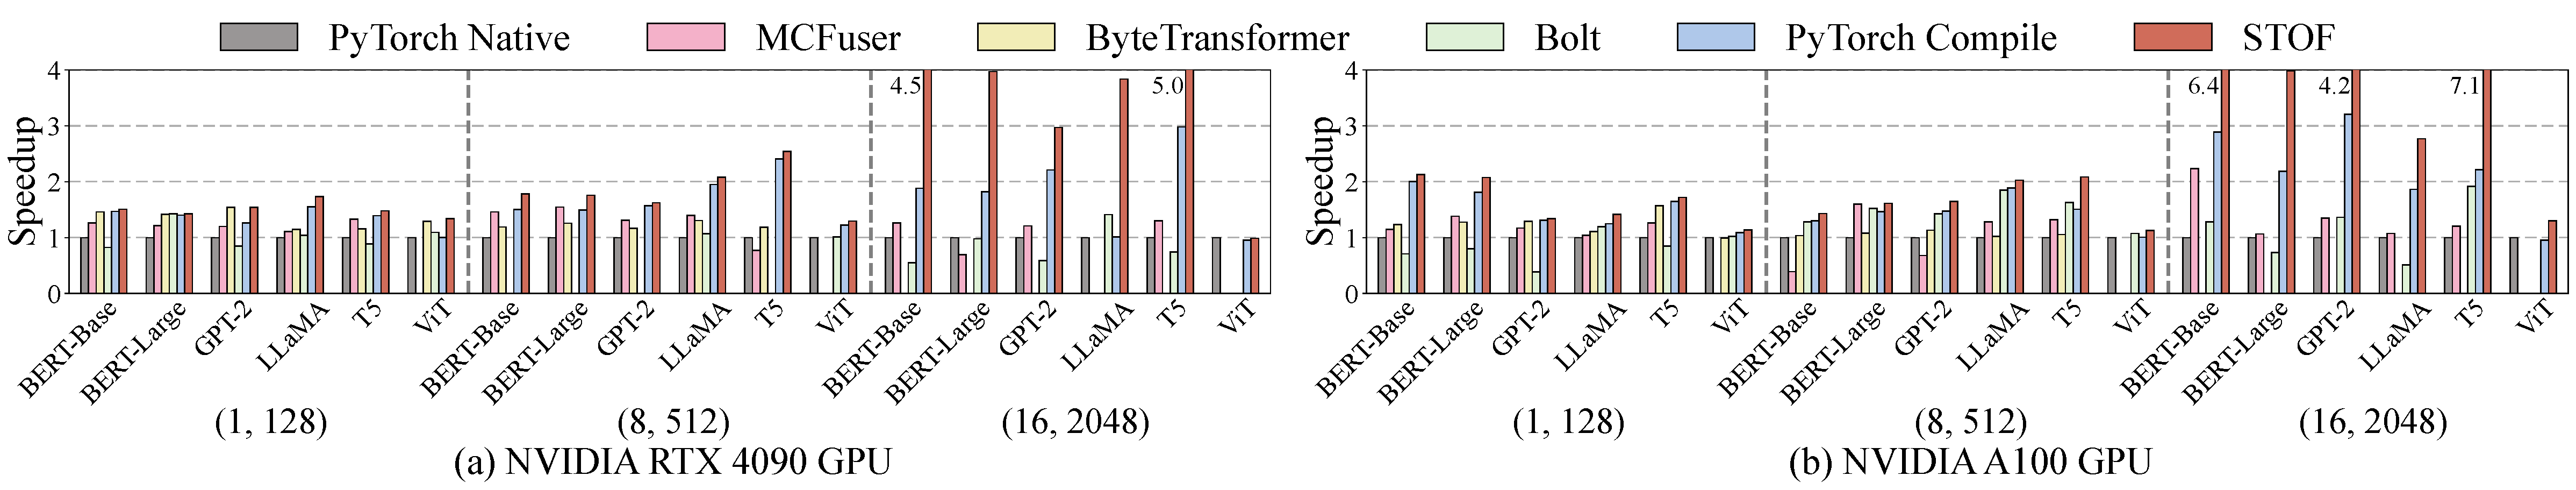
\includegraphics[width=\linewidth]{figures/5-eva-EE-4090-A100.pdf}
    \caption{The end-to-end performance of the methods normalized to that of PyTorch Native on RTX 4090 and A100 GPUs.}
    \label{fig:eva-EE-4090-A100}
\end{figure*}


\begin{table*}[htbp]
%\footnotesize
\scriptsize
\caption{Tuning time of STOF, MCFuser, and Bolt for end-to-end inference on A100 GPU in seconds.}
%\vspace{-8pt}
\centering 
\renewcommand{\arraystretch}{1.2}
\setlength{\tabcolsep}{2.7pt} % 列间距压缩到3pt
\begin{tabular}{|l||c|c|c|c|c|c||c|c|c|c|c|c||c|c|c|c|c|c|}
\hline
Input Size & \multicolumn{6}{c||}{(1, 128)}  & \multicolumn{6}{c||}{(8, 512)} & \multicolumn{6}{c|}{(16, 2048)} \\ \hline
Name &  BERT-B & BERT-L & GPT & LLaMA  & T5  & ViT  & BERT-B & BERT-L & GPT  & LLaMA  & T5  & ViT  & BERT-B & BERT-L & GPT   & LLaMA  & T5  & ViT \\ \hline \hline
MCFuser & 51.4   & 52.4   & 49.5 & 48.8 & 71.9 & 100.2  & 91.8   & 132.3   & 100.8 & 110.8 & 239.0 & 437.8  & 660.2   & 1049.7   & 664.4 & 820.6 & 1987.6 &  4264.3 \\ \hline
Bolt    & 53.3  & 57.3  & 48.8 &  52.1 & 70.7 &  120.7 & 90.8   & 126.1   & 99.8  & 124.6 & 244.7 &  468.8 & 652.2   & 1067.7   & 738.6 & 837.0 & 1860.8  & 3848.6 \\ \hline
STOF (ours)     & \textbf{23.3}   & \textbf{22.6}   & \textbf{23.8}  &  \textbf{29.5}  & \textbf{43.1}  &  \textbf{93.9}   & \textbf{40.9}   & \textbf{55.0}  & \textbf{40.9}  &  \textbf{43.6}  & \textbf{80.3} &  \textbf{99.3}  & \textbf{99.6}    & \textbf{225.3}     & \textbf{122.2} &  \textbf{264.6} & \textbf{388.3}   & \textbf{412.8} \\ \hline
\end{tabular}
\label{tab:tuning_time}
\end{table*}


% STOF 相比于 FlexAttn 的加速比还待算一下
\subsection{MHA Performance}
\label{sec:fusedMHA}


Figure~\ref{fig:MHA-evalaution-4090} and Figure~\ref{fig:MHA-evalaution-A100} present the MHA performance of the methods normalized to that of PyTorch Native on RTX 4090 and A100 GPUs. The missing bars are attributed to two reasons: 1) ByteTransformer lacks support for sequence lengths greater than 1,024; 2) MCFuser runs out of memory (OOM) when the input scale is large. As seen, STOF shows consistent superior performance on both GPU platforms.
Compared to the state-of-the-art FlexAttention implementation, STOF achieves the average speedups of 1.8$\times$ and 1.6$\times$ on RTX 4090 and A100 GPUs, respectively. 
STOF achieves superior performance on sliding window mask because its high sparsity and concentration of valid blocks facilitate computation skipping.
Even for causal masks, STOF still achieves a certain speedup over FA2 and FlexAttention under most cases. The reason is that the two-level storage format combining BSR and bitmap further improves on-chip memory locality. In contrast, due to the lack of tensor core support, SPLAT achieves decent performance on RTX 4090 GPU with higher CUDA core ratio, achieving a maximum speedup of 3.6$\times$ compared to PyTorch Native; but it lags behind on A100 GPU across all cases.



The above figures illustrate the MHA performance at different input scales in detail. At small scales, STOF achieves relatively better performance than FA2 and FlexAttention under most cases. STOF enables the row-wise kernel, where the use of shuffle operations within the warp incurs extremely low synchronization cost.
On the other hand, STOF achieves significant speedup compared to other methods at large input scales. For example, when the setting of (batch size, sequence length) is (16, 4,096), STOF achieves 4.8$\times$ and 4.9$\times$ speedups over FA2 and FlexAttention on A100 GPU, respectively. This is mainly because the block-wise kernel makes full use of the mask sparsity to skip unnecessary calculations. Besides, the optimizations such as asynchronous data copying and \textit{Q} register resident serve as the foundation for performance improvement.
Note that PyTorch Native, MCFuser, and ByteTransformer do not natively support sparse masks. The basic approach is to subtract the mask matrix, thus missing the opportunity to reduce the amount of calculation.

\subsection{End-to-end Performance}
\label{sec:end2end}

We benchmark five models including BERT-Base, BERT-Large, GPT2, LLaMA, T5 and ViT. Among them, BERT and ViT are encoder-only, GPT2 and LLaMA are decoder-only, whereas T5 contains both encoder and decoder. 
%These models serve as diverse workloads to evaluate the general applicability of the methods. 
We adopt the Bigbird mask and conduct experiments under three distinct settings of (batch size, sequence length): (1, 128), (8, 512), and (16, 2,048). Figure~\ref{fig:eva-EE-4090-A100} presents the end-to-end performance of the methods normalized to that of PyTorch Native on RTX 4090 and A100 GPUs. The missing bars indicate OOM for MCFuser or unsupported sequence length for ByteTransformer. As seen, STOF consistently delivers the highest speedups across the majority of models and settings on both GPU platforms. Even compared to the state-of-the-art PyTorch Compile, STOF achieves an average speedup of 1.3$\times$ and 1.4$\times$ on RTX 4090 and A100 GPUs, respectively. In addition to customizing the MHA kernel, the performance gain of STOF also comes from operator fusion and parameter tuning.

For the setting (16, 2,048), STOF achieves 1.5$\times$, 1.5$\times$, 1.2$\times$, 1.3$\times$, 1.1$\times$, and 1.2$\times$ speedups over PyTorch Compile for the six models on RTX 4090 GPU. A similar trend can be observed on A100 GPU. The results indicate that the advantages of STOF are particularly pronounced for larger input scales. The reason is attributed to the significant reduction in the absolute time of the bottleneck MHA computation. This demonstrates that STOF has the potential to be applied to future GPU generations with larger memory capacity.


\subsection{Tuning Cost}
\label{sec:search}
% 在正文中说明： BERT-B & BERT-L =   BERT-Base & BERT-Large



Table~\ref{tab:tuning_time} lists the tuning time of STOF, MCFuser, and Bolt for end-to-end inference on A100 GPU in seconds, where BERT-B/L is BERT-Base/Large. Note that PyTorch Native, PyTorch Compile, and ByteTransformer are not included due to the lack of tuning support. As seen, the tuning time of STOF is less than that of MCFuser and Bolt in all cases. This advantage becomes more prominent when the input scale is large. Since the tuning process of operator fusion module in STOF is positively correlated with the input tensor, the tuning cost per iteration increases moderately, but it does not grow linearly with respect to the overall tuning time. For the setting (16, 2,048), STOF is on average 6.7$\times$ and 6.9$\times$ faster than MCFuser and Bolt. This is mainly because reward-based sampling enables STOF to find high-performance settings in a shorter time. On the other hand, the caching mechanism ensures that the same parameter setting in each fusion scheme will not be executed repeatedly, which particularly saves tuning time in scenarios with large input scales.
%This is particularly effective in saving tuning time, especially in 




\subsection{Ablation Study}
\label{sec:ablation}

%To understand the individual contributions of the key modules of our proposed method, we conduct an ablation study. 
Figure~\ref{fig:5-ablation} presents the speedup of STOF with only unified MHA module or only operator fusion module over PyTorch Native and PyTorch Compile on A100 GPU. 
For reference, the speedup of STOF with both modules is also shown in the figure. For PyTorch Compile, we also break the MHA boundary, transforming the whole computation graph into low-level meta operators for compilation optimization.


As seen, the operator fusion module contributes more to the performance when the input scale is small. Taking the setting of (1, 128) as an example, the speedup achieved by only fusion module is 19.5\% higher than that of only MHA module on average. In fact, the low sequence length and batch size lead to a small computational workload, which is particularly friendly to the fusion of CI operators. However, the contribution of the MHA module exceeds that of fusion module as the input scale increases. For the (16, 2,048) setting, the speedup of only MHA module is 2.0$\times$ on average, higher than that of only fusion module. Since MHA computation becomes the bottleneck, the high parallelism of the block-wise kernel is reflected in end-to-end inference. Note that STOF with both modules always achieves the highest speedup, indicating that the optimizations can complement each other. 
On the other hand, we find that breaking the MHA boundary would compromise these tailored kernel optimizations. The results show that such boundary breaking causes up to 1.5$\times$ slowdown compared to preserving it.

% PyTorch Compile without MHA boundary 与 PyTorch Compile 相比；慢了 1.5x

%To further investigate the performance implications of MHA fusion boundaries, we designed the ``PyTorch Compile with broken MHA boundary'' cases for comparison. Breaking the MHA boundary to fuse the GEMM with other operators would compromise these tailored kernel optimizations. 



% SQX: 顺序换一下，三个baseline放前面，调整为：PyTorch Native、PyTorch Compile、PyTorch Compile without MHA boundary、Only MHA Module、Only Fusion Module、MHA Module+Fusion Module。
\begin{figure}[htbp]
    \centering
    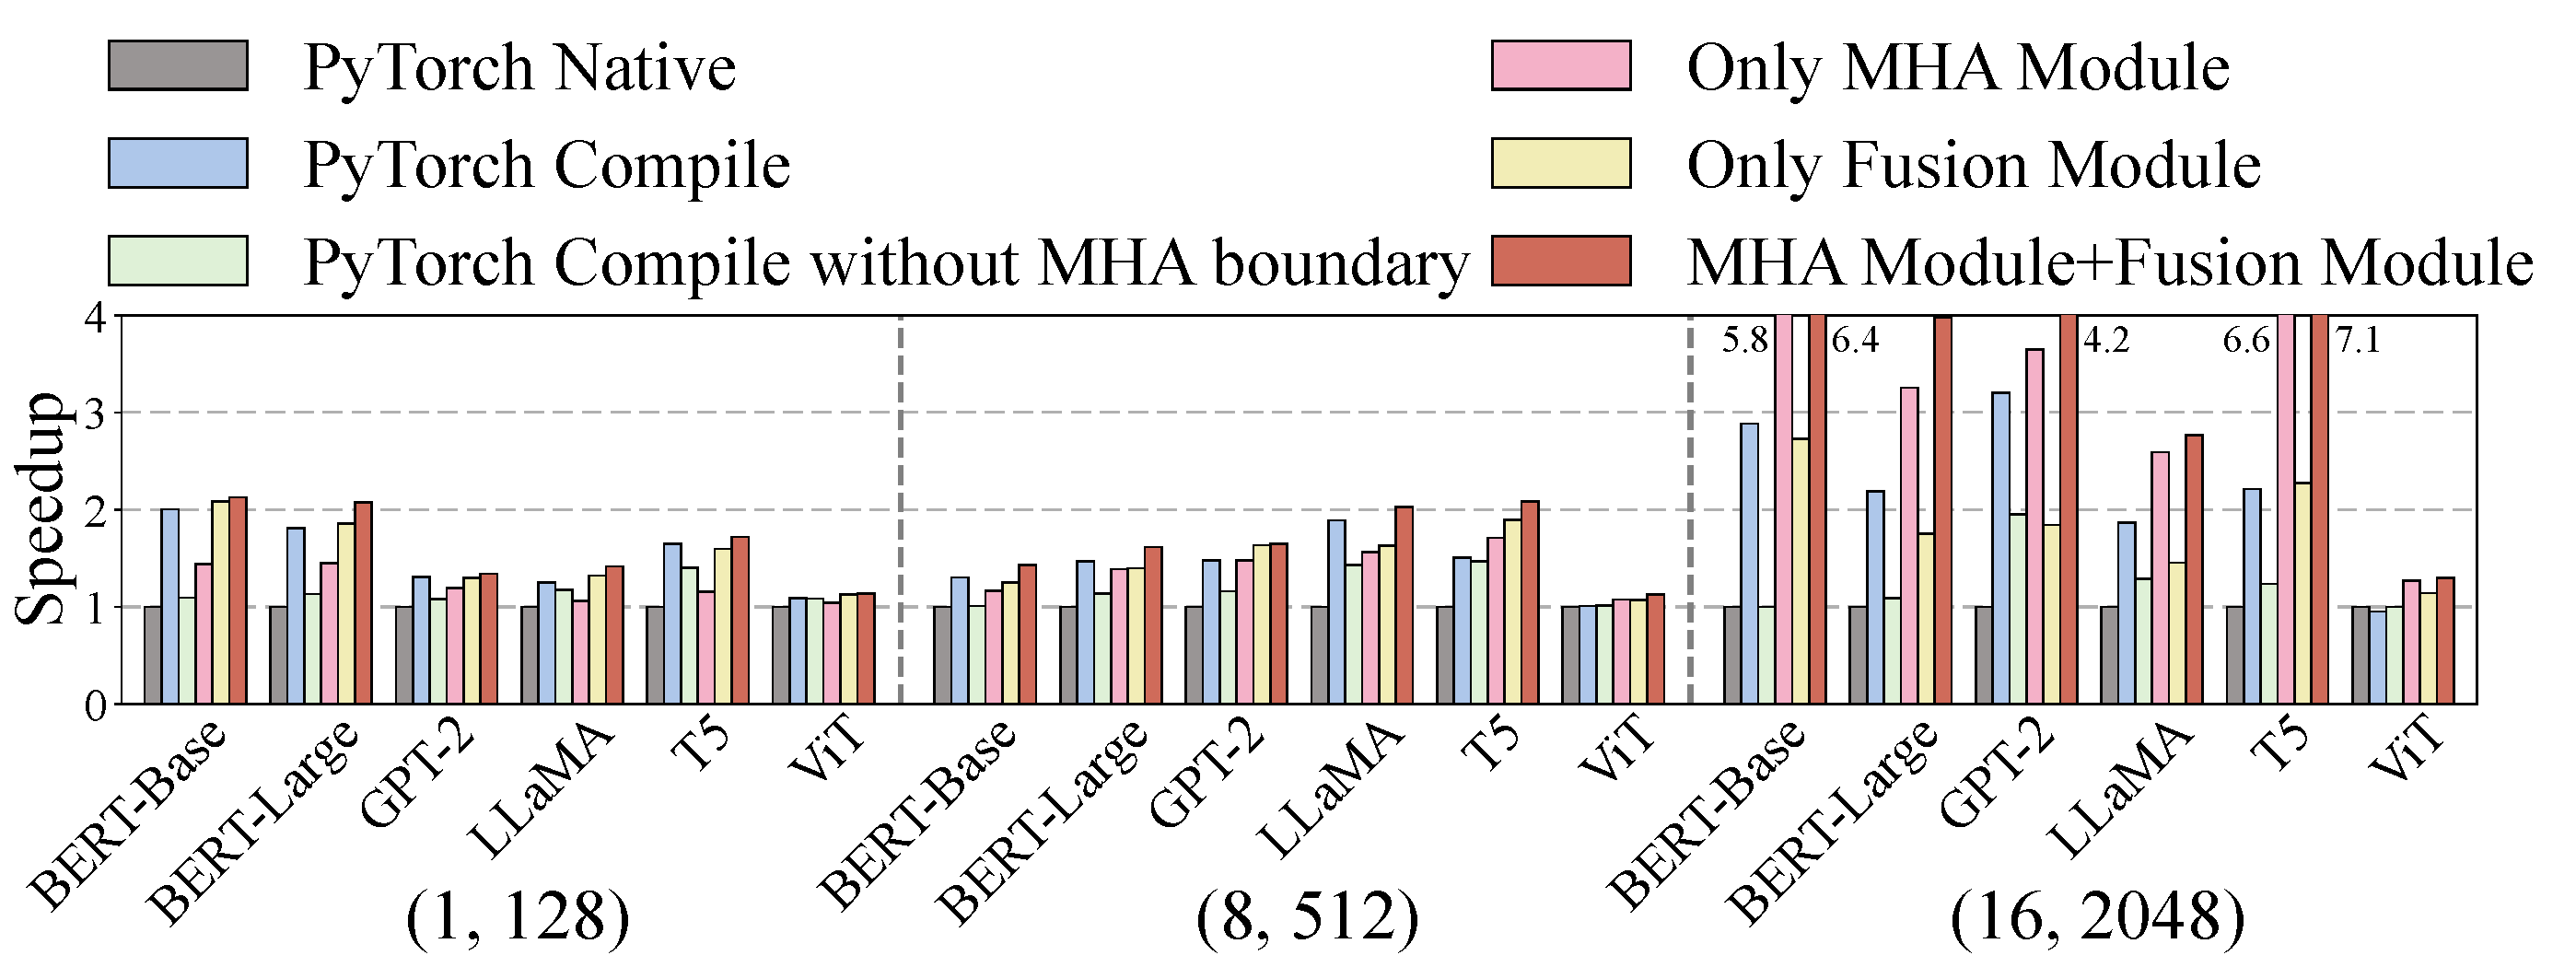
\includegraphics[width=\linewidth]{figures/5-Percentage.pdf}
    %%\vspace{-10pt}
    \caption{The speedup of STOF with only MHA module or only fusion module over PyTorch Native on A100 GPU.}
    \label{fig:5-ablation}
\end{figure}



\subsection{Overhead Analysis}
\label{sec:overhead}

The STOF overhead mainly includes the analysis model, scheme conversion (i.e., hash encoding and numerical decoding), and reward algorithm. The analysis model is reflected in MHA kernel selection and fusion scheme initialization. Figure~\ref{fig:5-Percentage} presents the time breakdown of STOF overhead normalized to the tuning process on A100 GPU. As seen, the time proportion of scheme conversion and reward algorithm is relatively smaller when the input scale is large. This is because these overheads are dominated by the model structure, and a larger input scale will lead to a longer tuning time, thus diluting this proportion. In contrast, the proportion of analytical model increases with the input scale. The primary reason is that the overhead for analyzing mask blocks increases with longer sequence lengths. Nevertheless, the analysis constitutes at most 0.5\% of the total time. Overall, STOF accounts for less than 3\% of the total tuning time, making it highly acceptable in the context of model fine-tuning.


\begin{figure}[htbp]
    \centering
    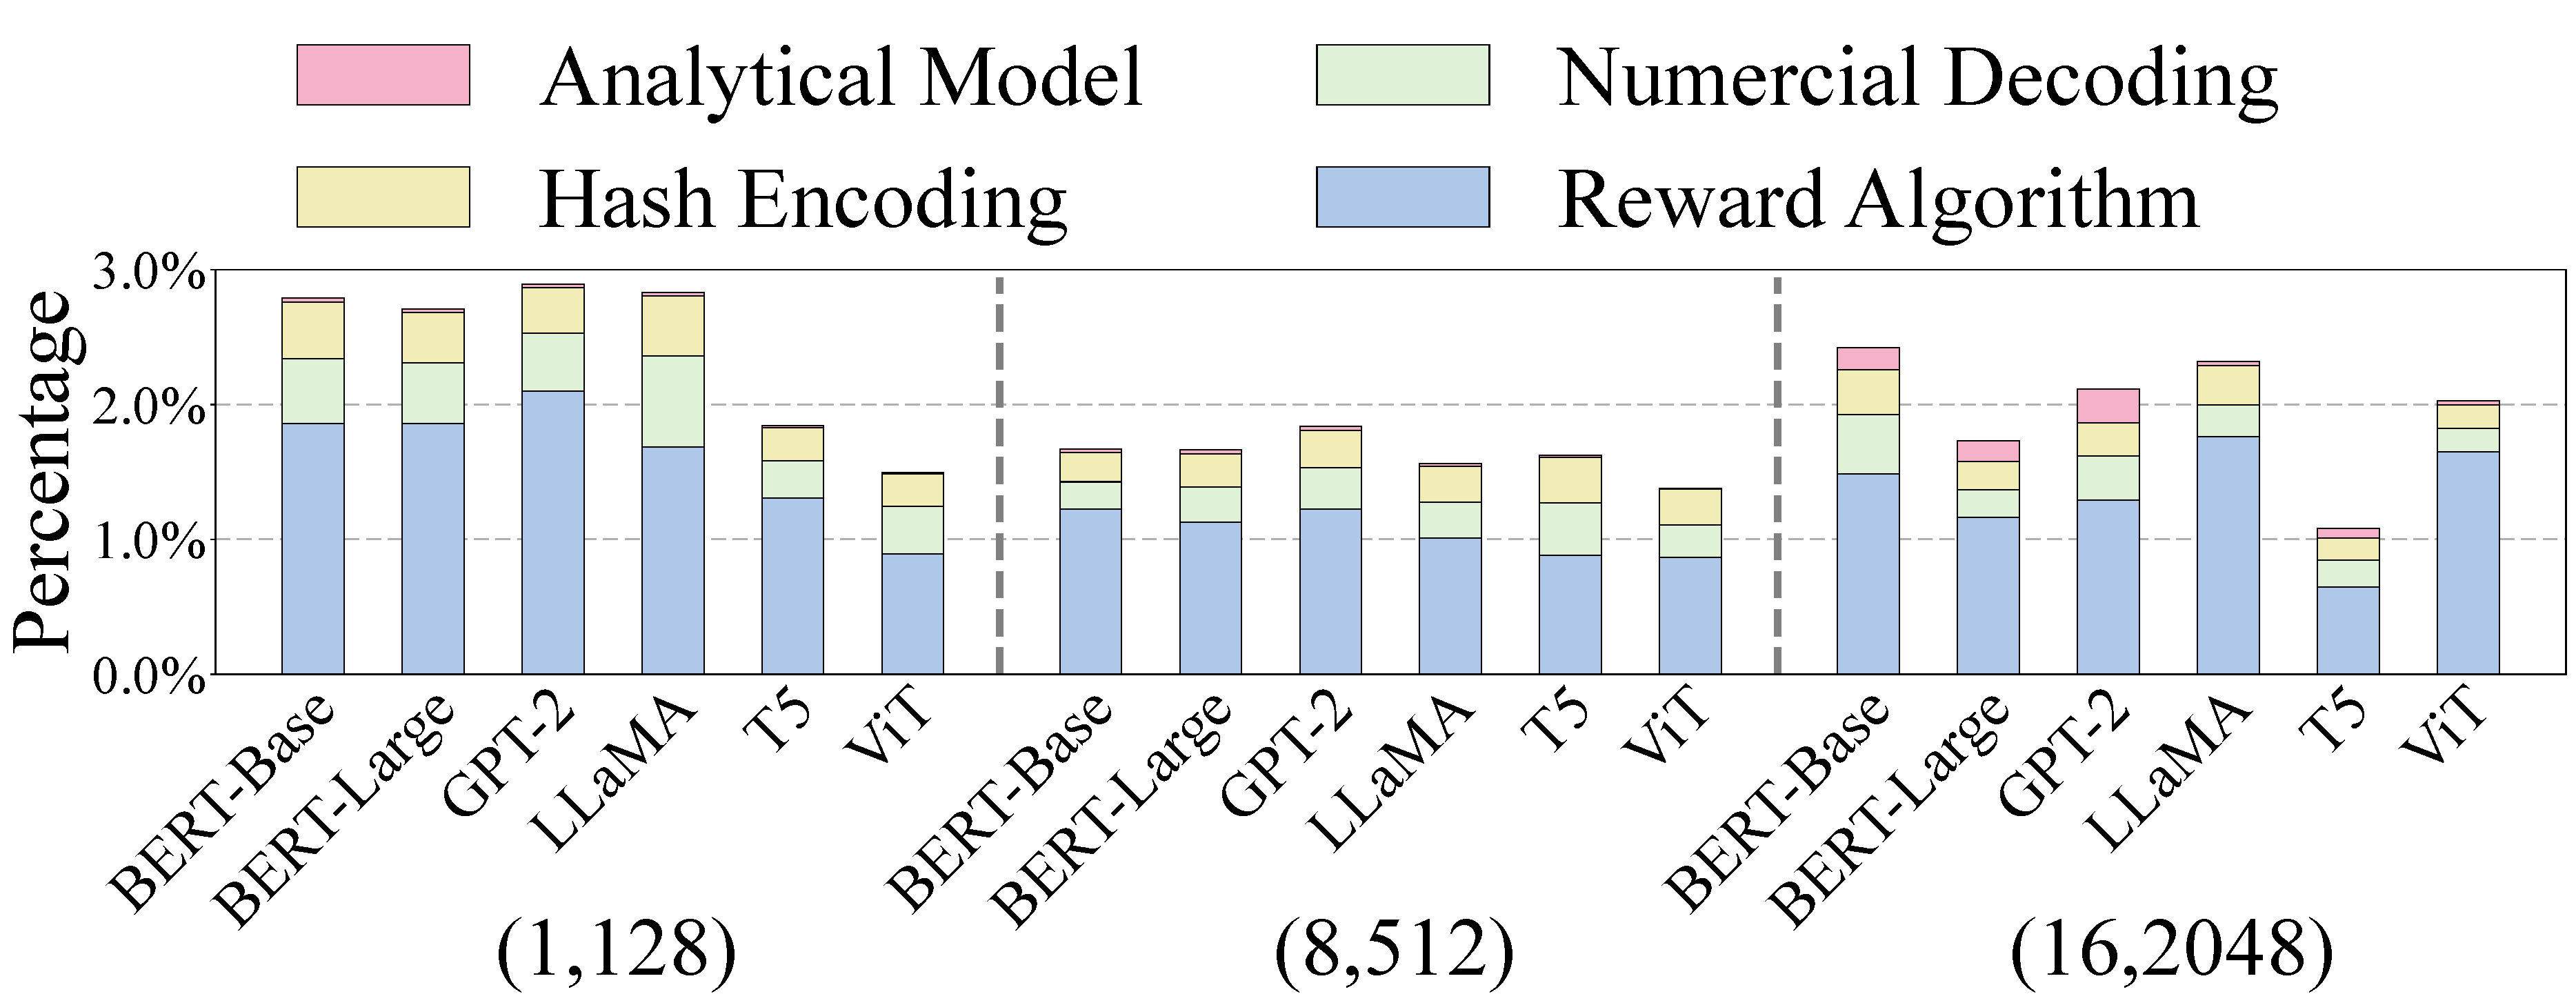
\includegraphics[width=\linewidth]{figures/5-ablation.pdf}
    %%\vspace{-10pt}
    \caption{Time breakdown of the STOF overhead normalized to the tuning process on A100 GPU.}
    \label{fig:5-Percentage}
\end{figure}

\subsection{Discussion}
\label{sec:discussion}
% Evaluation on longer sequence length
% Newer NVIDIA architectures
% Support for dynamic sparse patterns

\subsubsection{Newer GPU Architectures}

In addition to NVIDIA Ampere and Ada architectures, we have conducted preliminary tests on newer hopper architecture (i.e., NVIDIA H20 GPU). The results show that STOF consistently outperforms FA2, achieving up to 1.4$\times$ speedup for MHA computation. This proves that kernel optimizations of STOF are universal across GPU architectures. We plan to extend this evaluation to include FA3 for future work.

%hardware. Results on the NVIDIA H20 GPU demonstrate that STOF consistently outperforms FA2, achieving up to 1.4$\times$ speedup. We plan to extend this evaluation to include FA3 on Hopper architecture in future work. 

\subsubsection{Longer Sequence Lengths}

% SQX: 补充一下xx
We explore sequence lengths ranging from 4k to 16k and batch size of 1 on NVIDIA A100 GPU. STOF achieves significant speedups over the SOTA PyTorch Compile, reaching 4.1$\times$, 11.1$\times$, and 16.8$\times$ at 4k, 8k, and 16k, respectively. In addition, all baselines except STOF encounter Out-of-Memory (OOM) errors at sequence length of 32k, whereas STOF reaches OOM at 64k. The results indicate that STOF exhibits greater performance improvement for ultra-long sequence lengths, as well as significantly saving GPU memory.

%Additionally, we explore longer sequence lengths from 4k to 16k on NVIDIA A100 40GB GPUs. While all baselines except STOF encounter Out-of-Memory (OOM) errors beyond 32k sequence length (STOF reaches OOM at 64k), STOF achieves significant speedups over the SOTA PyTorch Compile, reaching 4.1$\times$, 11.1$\times$, and 16.8$\times$ at 4k, 8k, and 16k, respectively.

\subsubsection{Dynamic Mask Patterns}

STOF is inherently positioned to support dynamic mask patterns due to its flexible design. For example, MInference~\cite{jiang2024minference} could serve as a sophisticated frontend to discover dynamic patterns, with STOF as the execution backend. The main challenge lies in efficiently integrating MInference's offline pattern determination and online index generation into STOF's compilation pipeline with minor overhead. For future work, we plan to extend the analytical model to determine optimal configurations at runtime based on input token sequence.



